
\section{Device Frabrication}

\subsection{PDMS channels}

\begin{figure}[h]
    \centering
    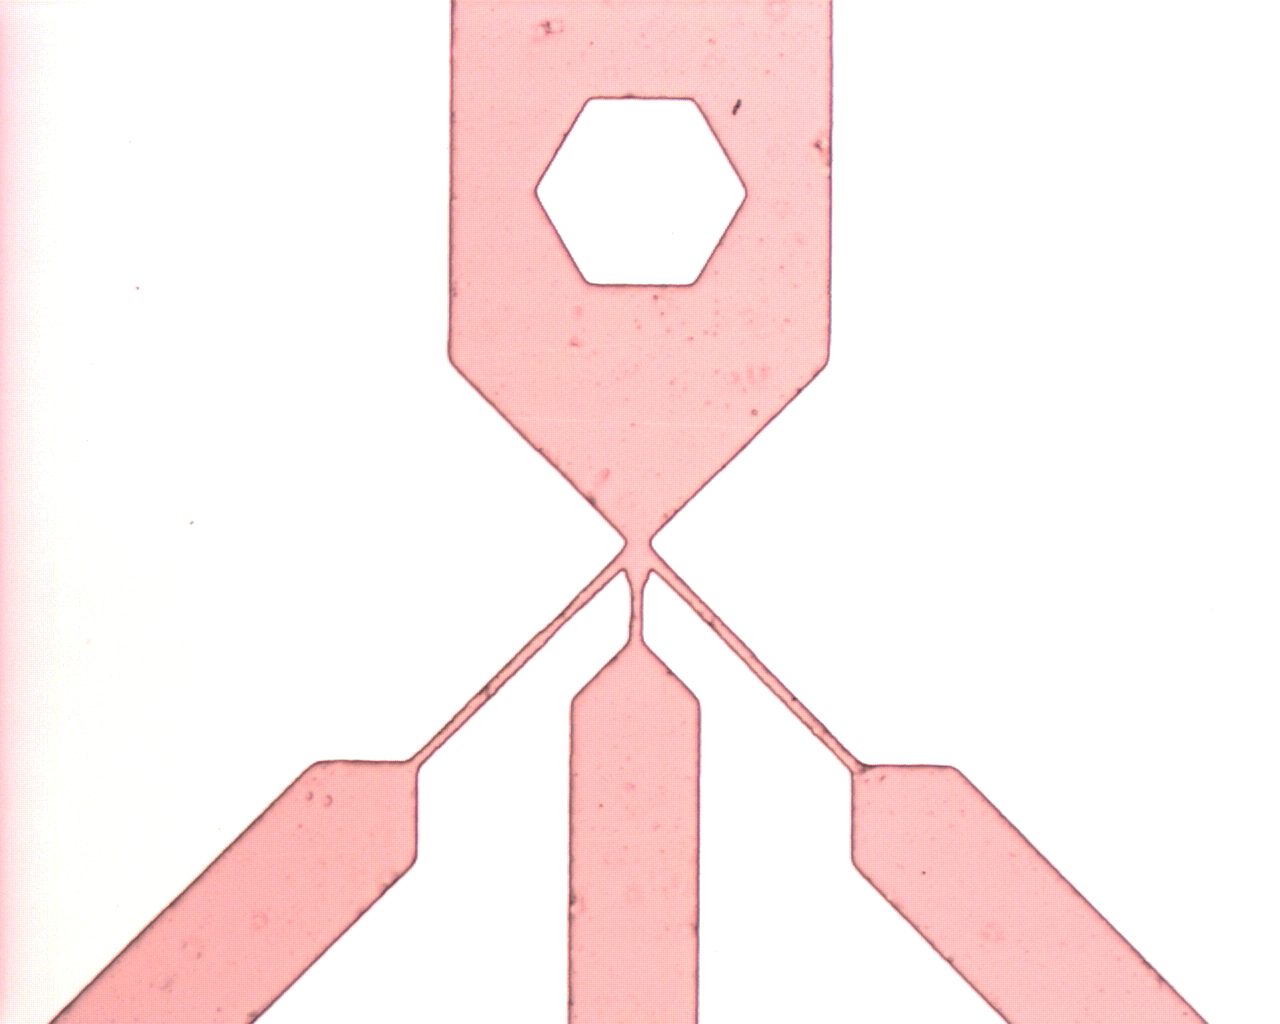
\includegraphics[width=\textwidth]{images/su8_results.png}
    \caption{SU-8 photoresist on the master mold.}
    \label{fig:su8_results}
\end{figure}

\begin{figure}[h]
    \centering
    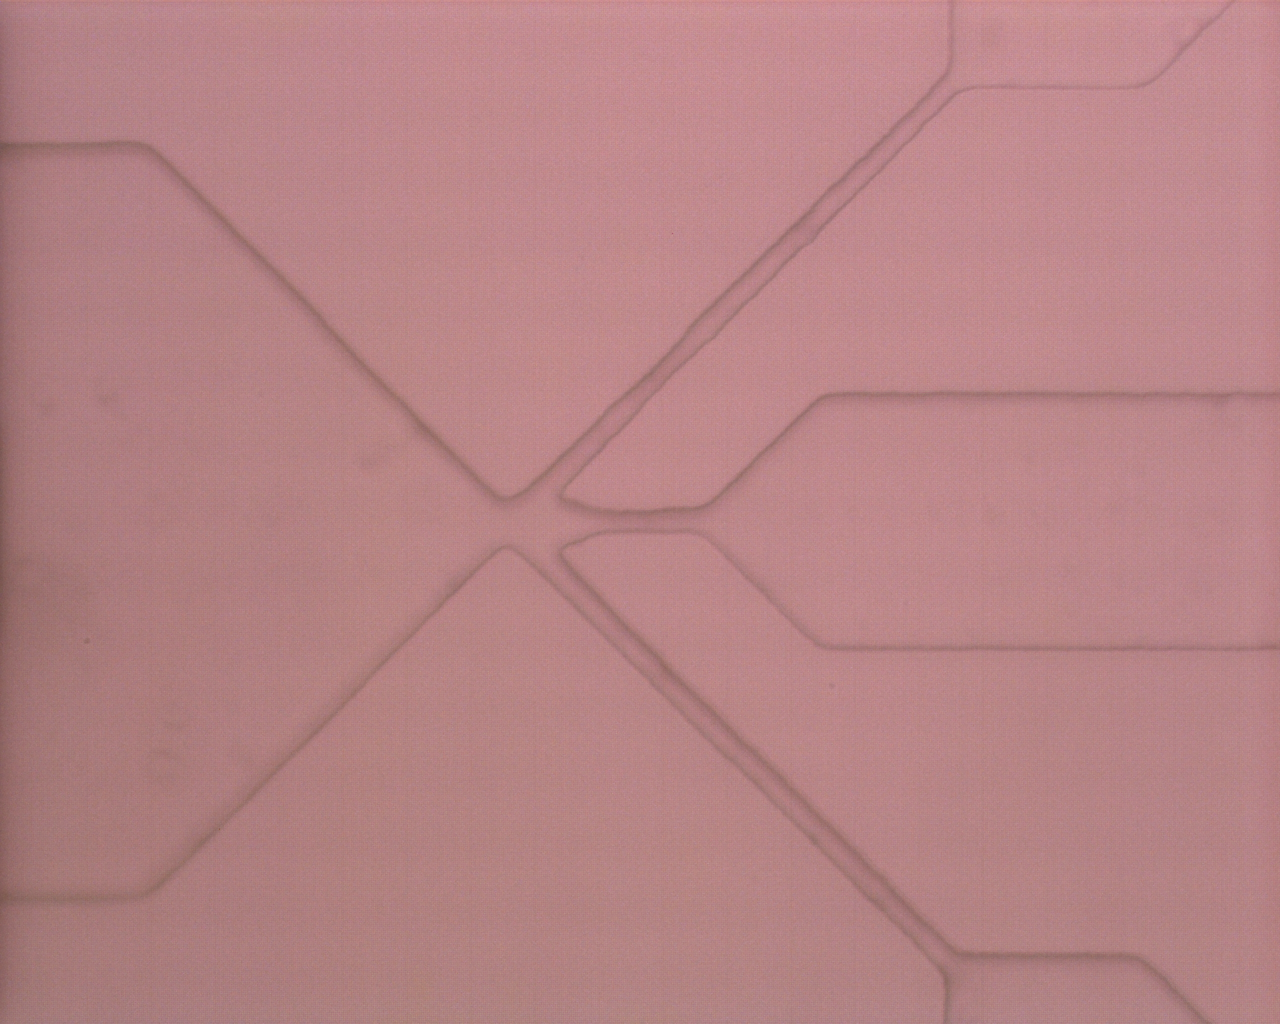
\includegraphics[width=\textwidth]{images/PDMS_channels.png}
    \caption{PDMS cast from the master mold.}
    \label{fig:pdms_results}
\end{figure}

\begin{figure}[h]
    \centering
    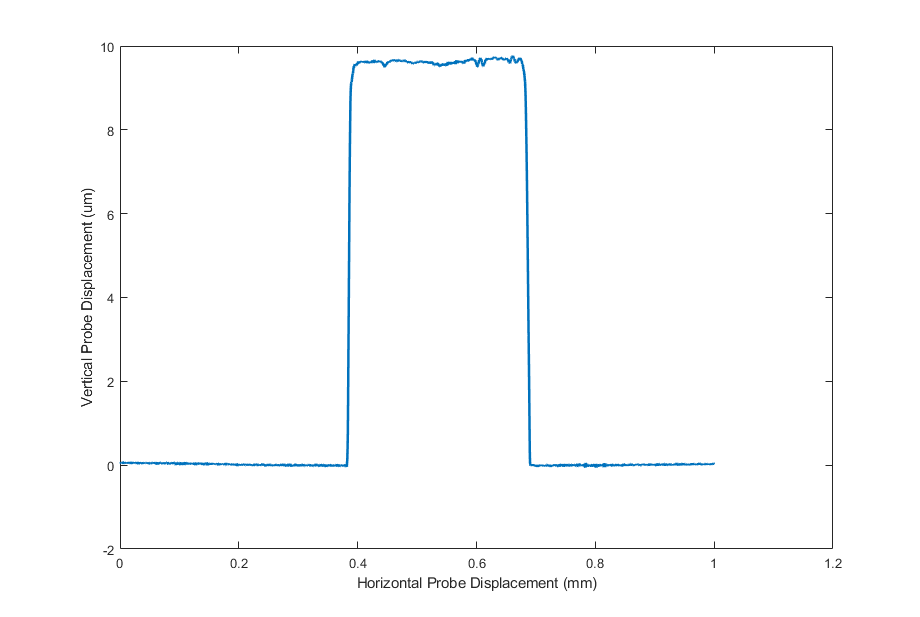
\includegraphics[width=\textwidth]{images/300umWideChannel.png}
    \caption[Surface profile of a 300 micron wide channel on the SU-8 master mold.]{Surface profile of a 300 micron wide channel on the SU-8 master mold. The profile was captured with the Ambios XP-1 profilometer. The profilometer recorded a channel height of 9.6 microns.}
    \label{fig:profilometer_300um_channel}
\end{figure}

\begin{figure}[h]
    \centering
    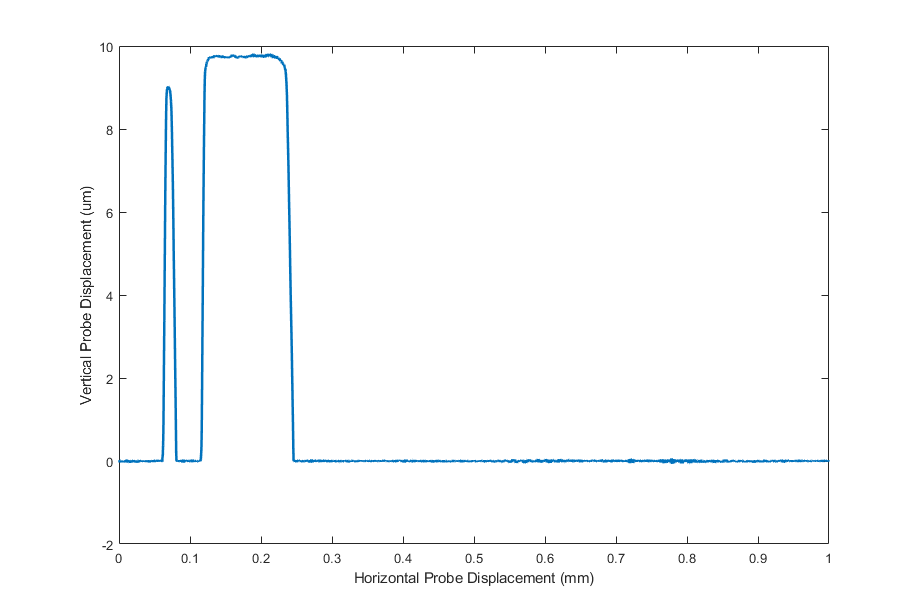
\includegraphics[width=\textwidth]{images/10umWideAndSidewaysThrough100umWide.png}
    \caption[Surface profile of a 10 micron and 100 micron wide channel on the SU-8 master mold.]{Surface profile of a 10 micron and 100 micron wide channel on the SU-8 master mold. The profile was captured with the Ambios XP-1 profilometer. The data depicts the 100 micron channel as about 140 microns wide since it crossed the channel at 45$^\circ$ The profilometer recorded a channel height of 9 and 9.6 microns for the 10 micron and 100 micron channels respectively.}
    \label{fig:profilometer_10um_channel_100um_sideways}
\end{figure}


\FloatBarrier


\subsection{Electrode Fabrication}

\begin{figure}[h]
    \centering
    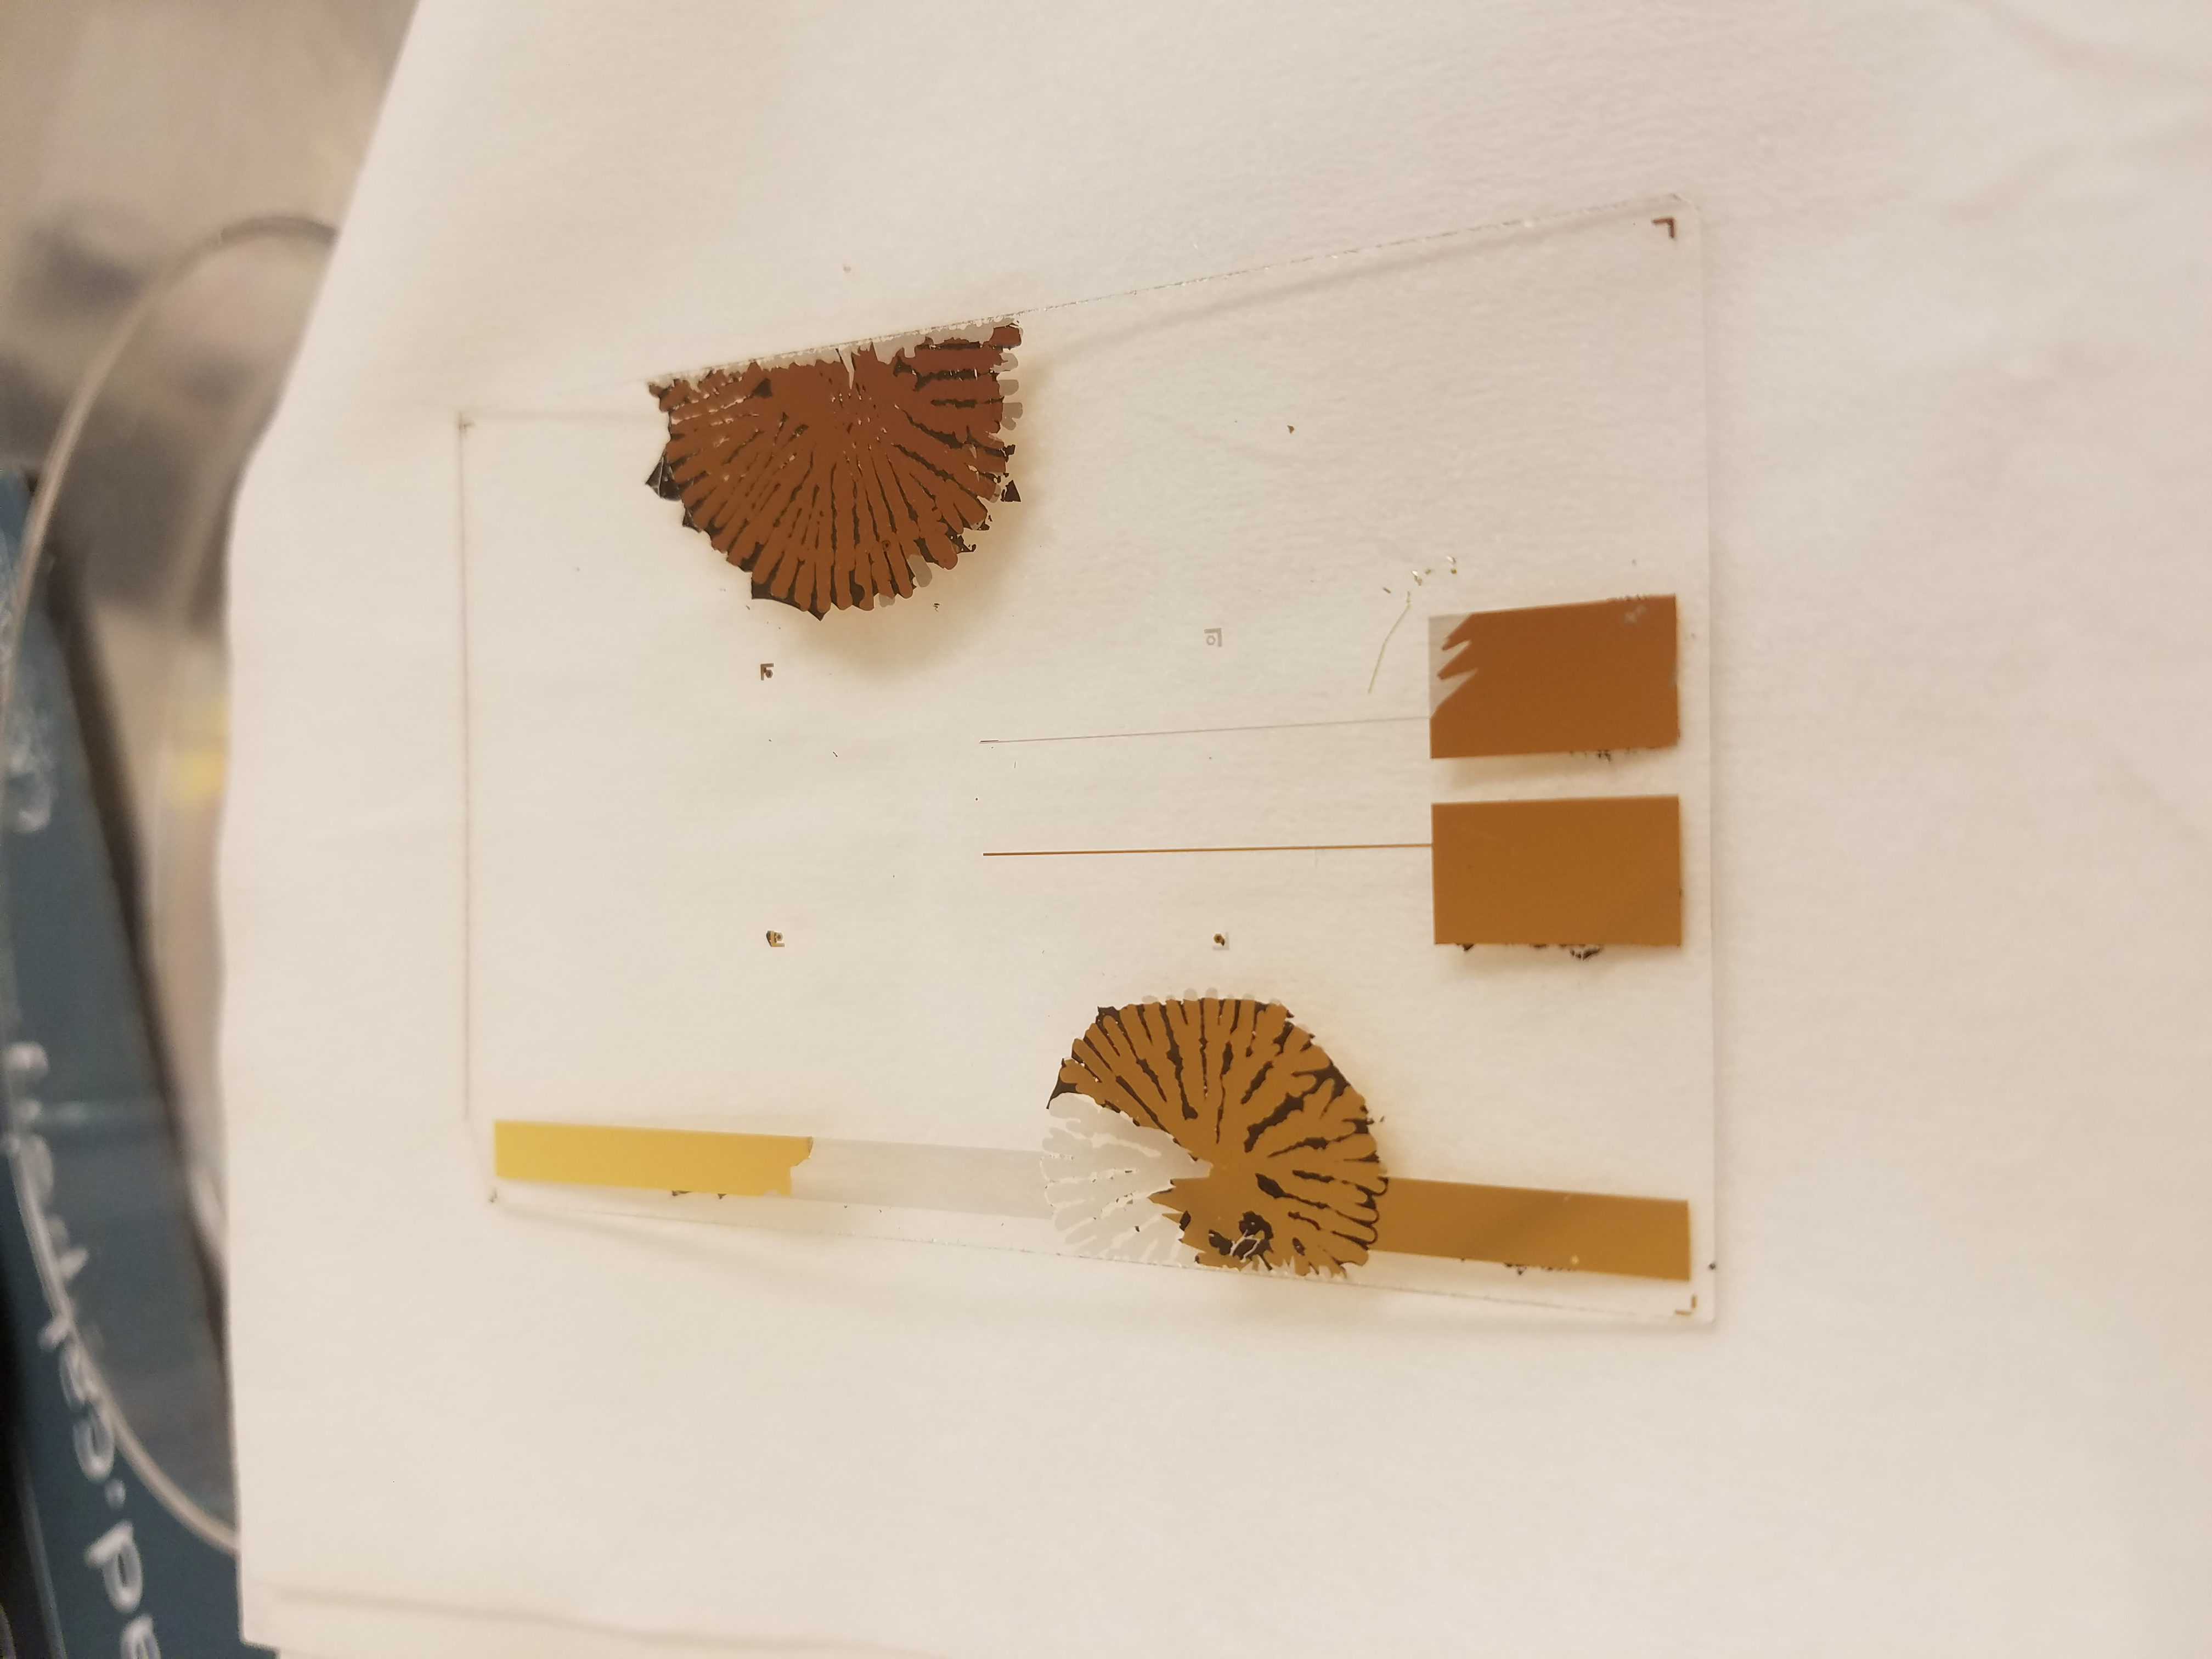
\includegraphics[width=\textwidth]{images/adhesion_issues.jpg}
    \caption{Electrode fabrication failure demonstrating two modes of failure: the ?? photoresist failed to properly adhere to the glass surface manifesting as two anomalous flower patterns, and poor adhesion of the deposited gold to the first chrome layer as evident by gold-stripped leads.}
    \label{fig:failed_electrode_macro}
\end{figure}

\begin{figure}[h]
    \centering
    \begin{subfigure}[b]{0.45\textwidth}
        \centering
        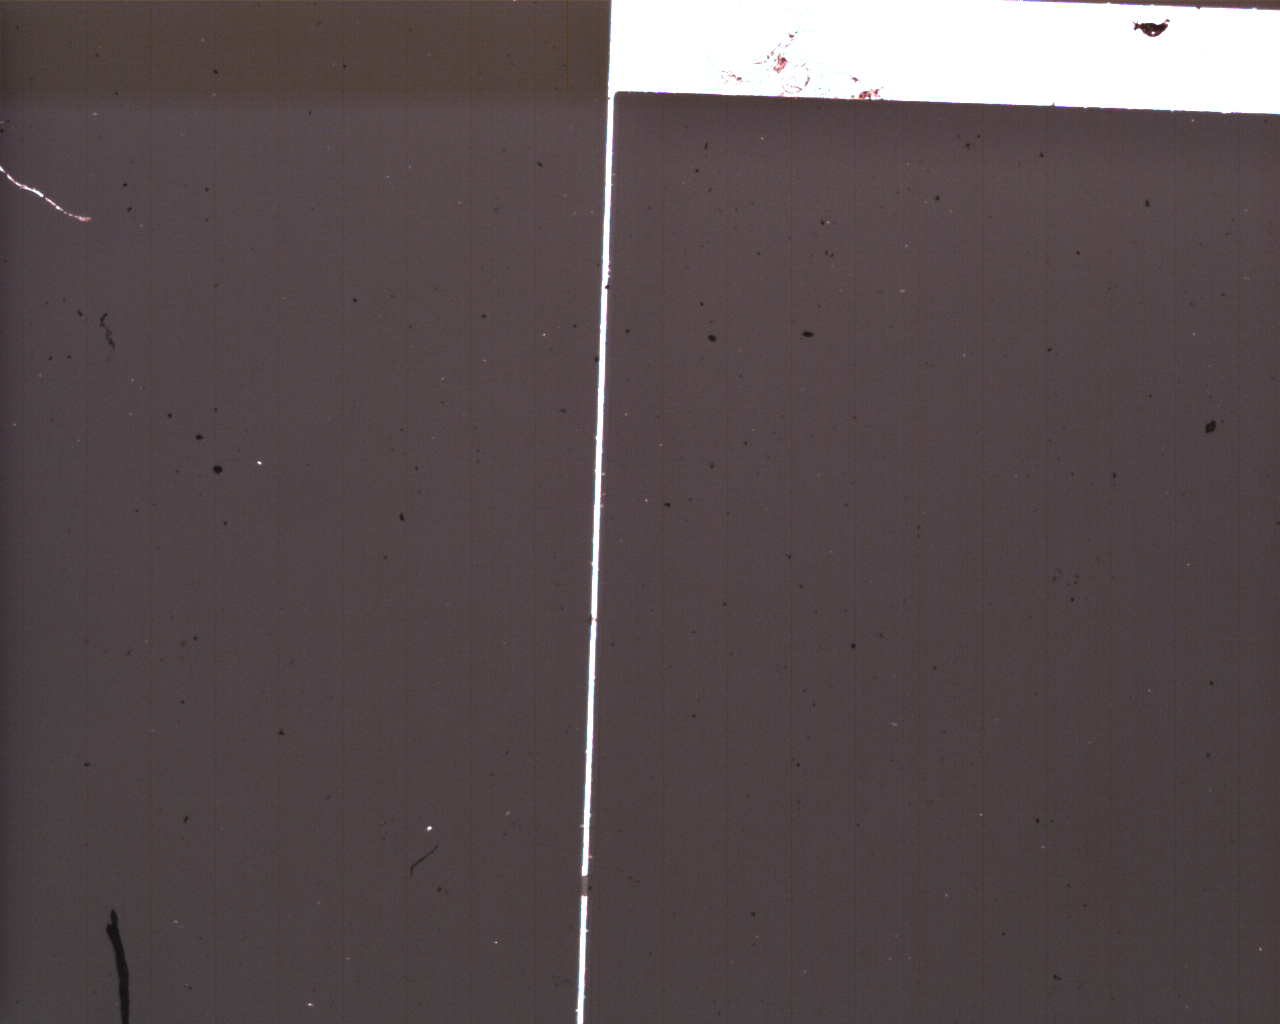
\includegraphics[width=\textwidth]{images/electrodeFailureChunkBreak.png}
        \caption{Impedance magnitude and phase}
    \end{subfigure}
    \hfill
    \begin{subfigure}[b]{0.45\textwidth}
        \centering
        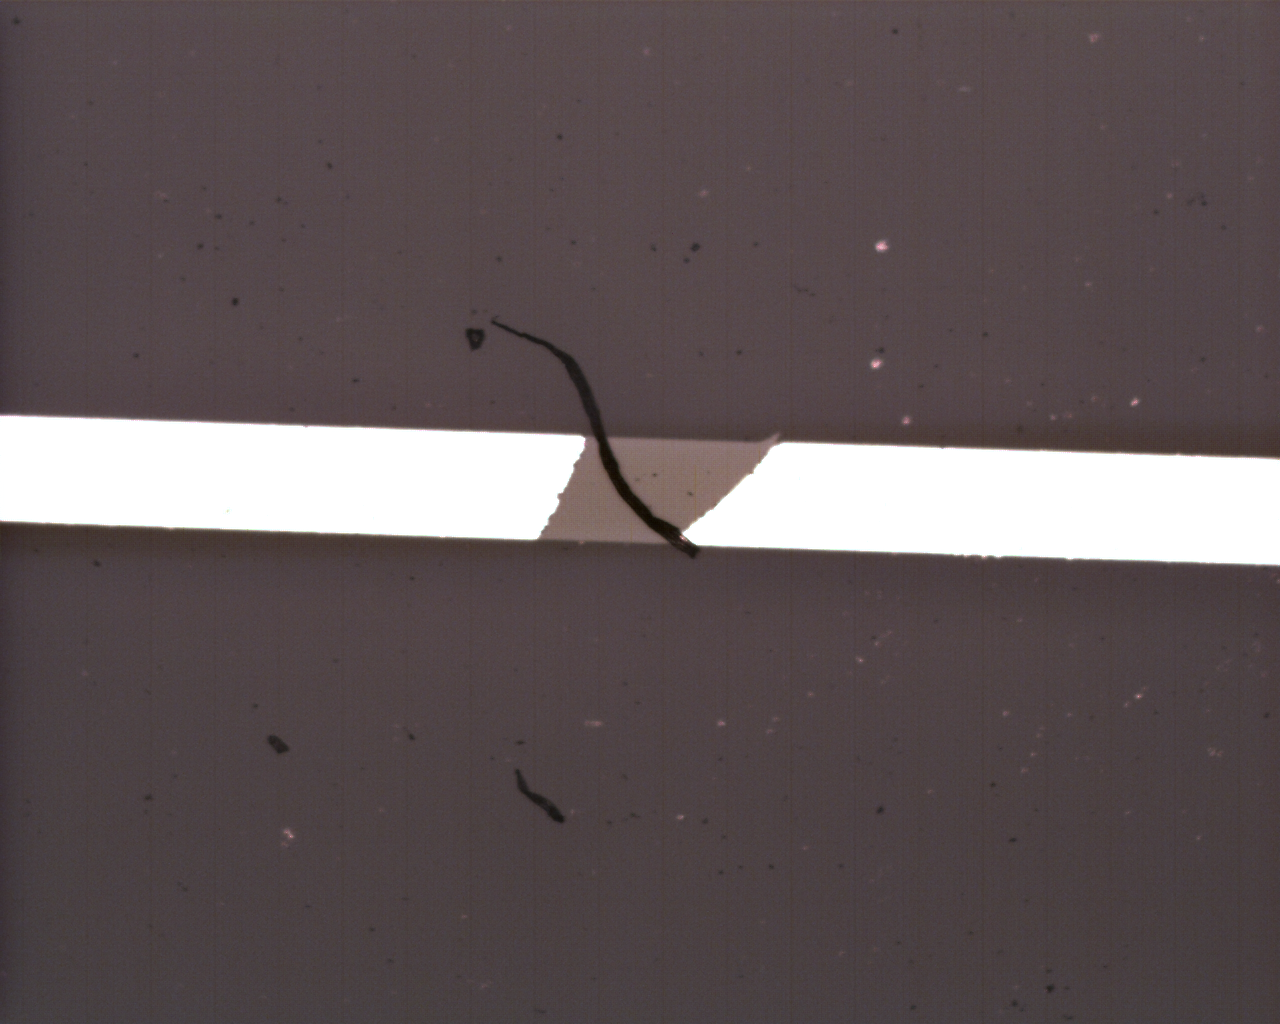
\includegraphics[width=\textwidth]{images/electrodeFailureChunkBreakZoomed.png}
        \caption{Real and imaginary impedance}
    \end{subfigure}
    \\
    \vspace{0.1 in}
    \begin{subfigure}[b]{0.45\textwidth}
        \centering
        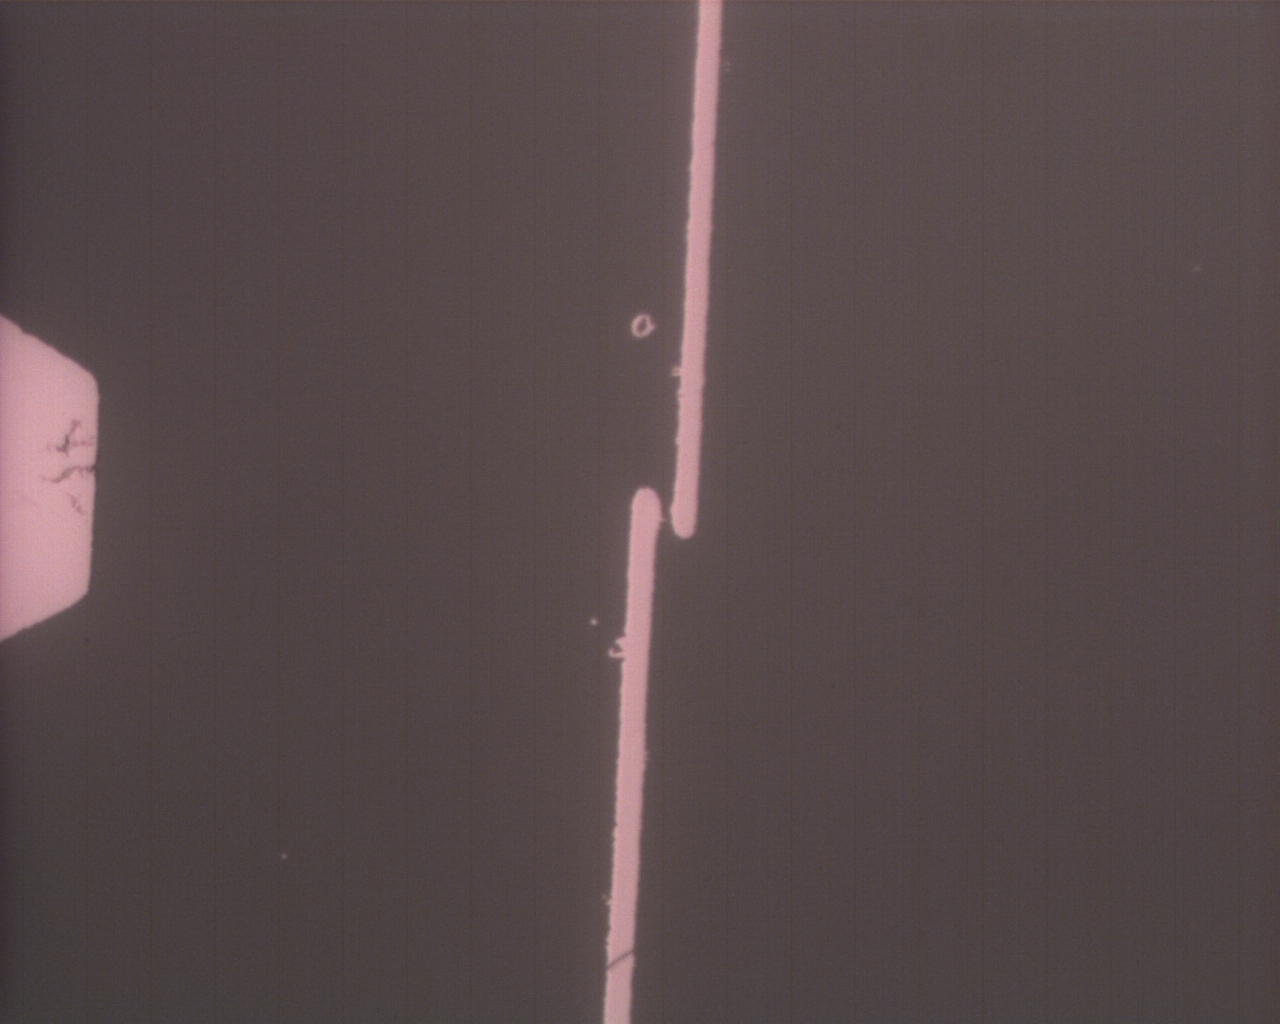
\includegraphics[width=\textwidth]{images/electrodeFailureThinBreak.png}
        \caption{Nyquist plot}
    \end{subfigure}
    \hfill
    \begin{subfigure}[b]{0.45\textwidth}
        \centering
        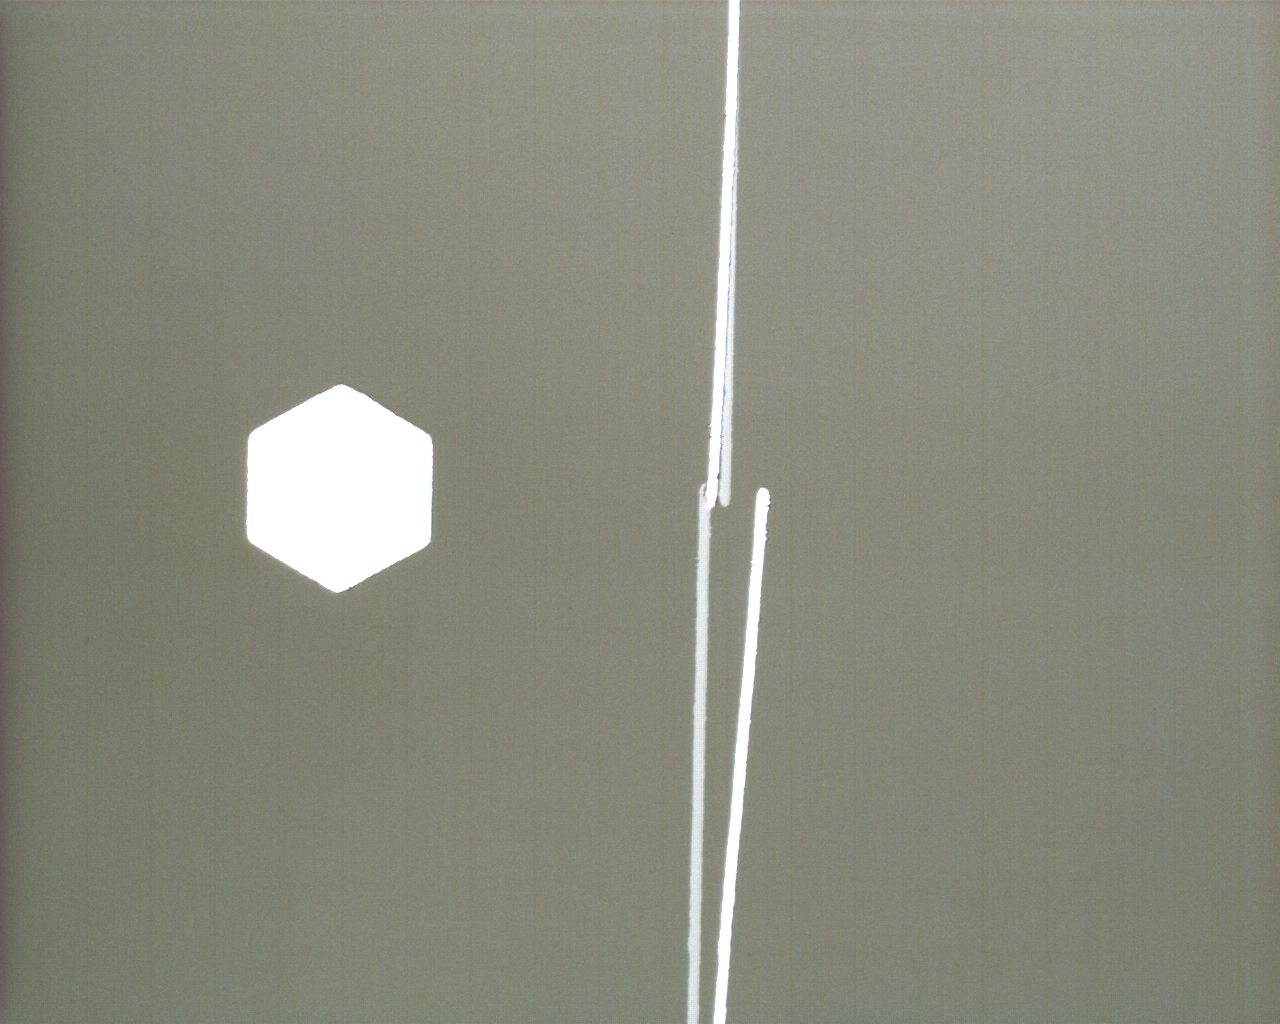
\includegraphics[width=\textwidth]{images/electrodeFailureSlide.png}
        \caption{Clausius Mossotti Factor}
    \end{subfigure}
    \caption{Example plots depicting results of the analytic impedance solution generated by the IS App.}
    \label{fig:failed_elecftrodes_micro}
\end{figure}

\begin{figure}[h]
    \begin{subfigure}[b]{\textwidth}
        \centering
        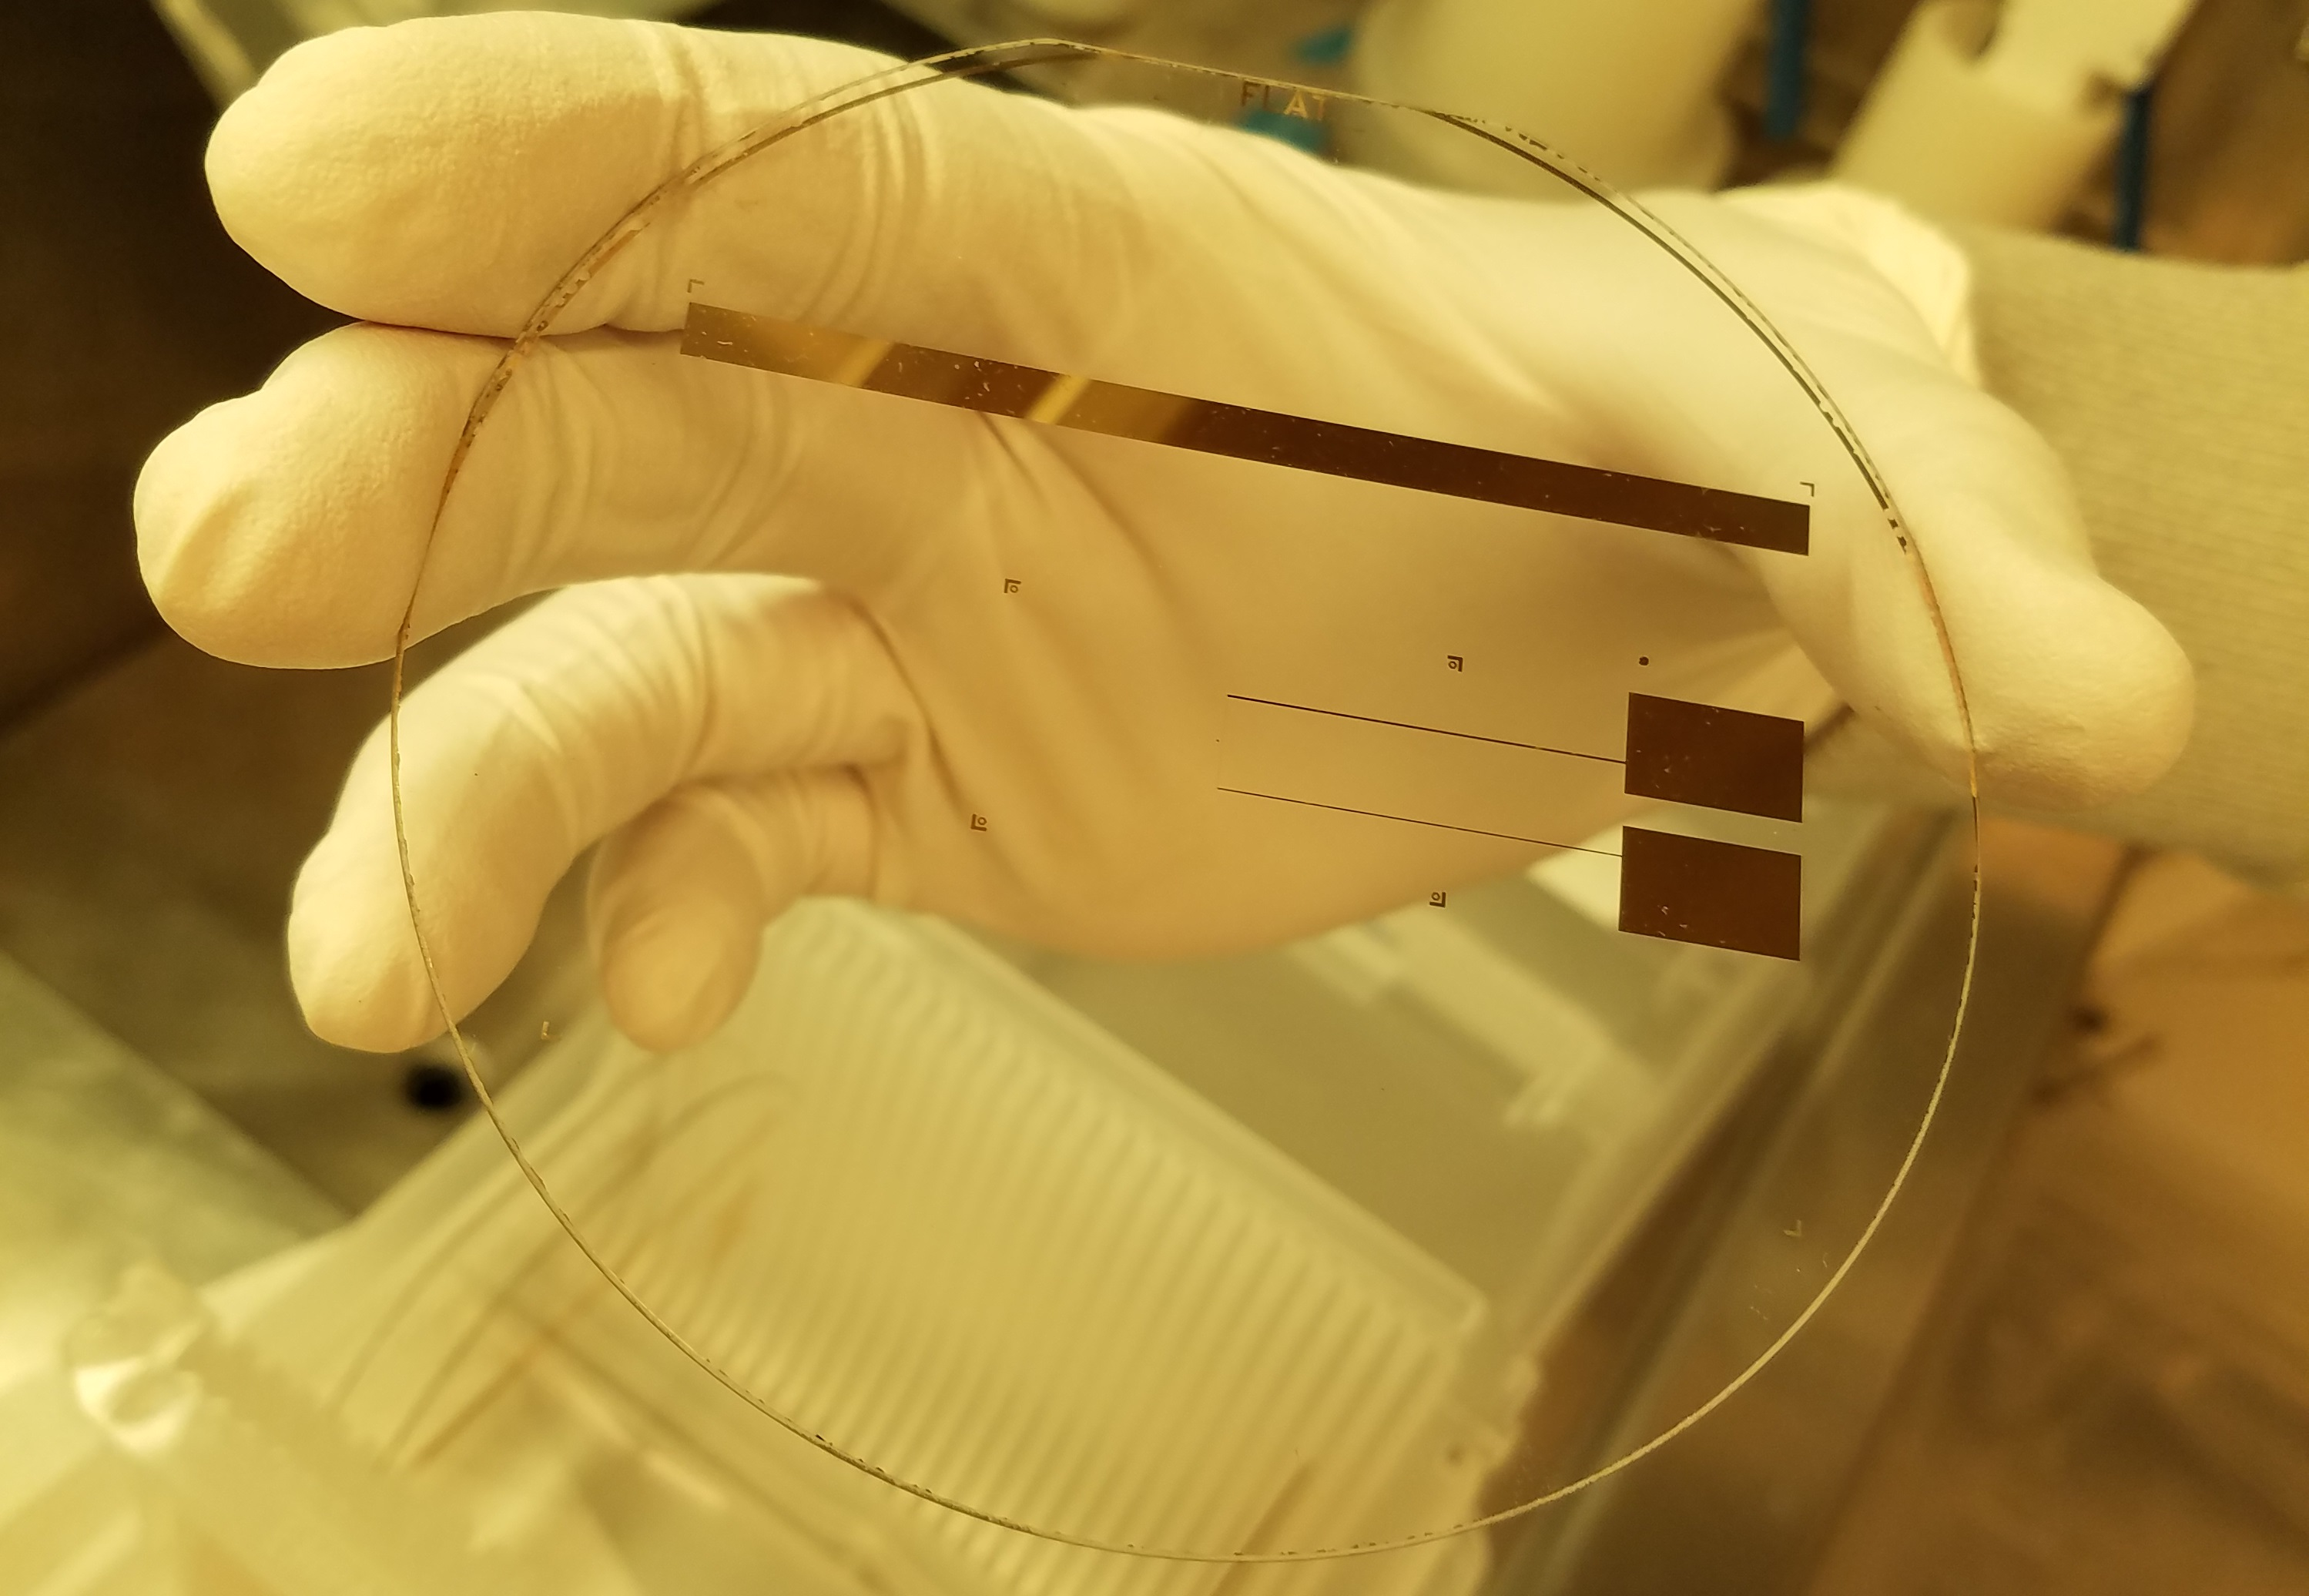
\includegraphics[width=\textwidth]{images/electrodes_real.jpg}
        \caption{Successful fabrication of device electrodes}
    \end{subfigure}
    \\
    \vspace{0.1 in}
    \centering
    \begin{subfigure}[b]{0.45\textwidth}
        \centering
        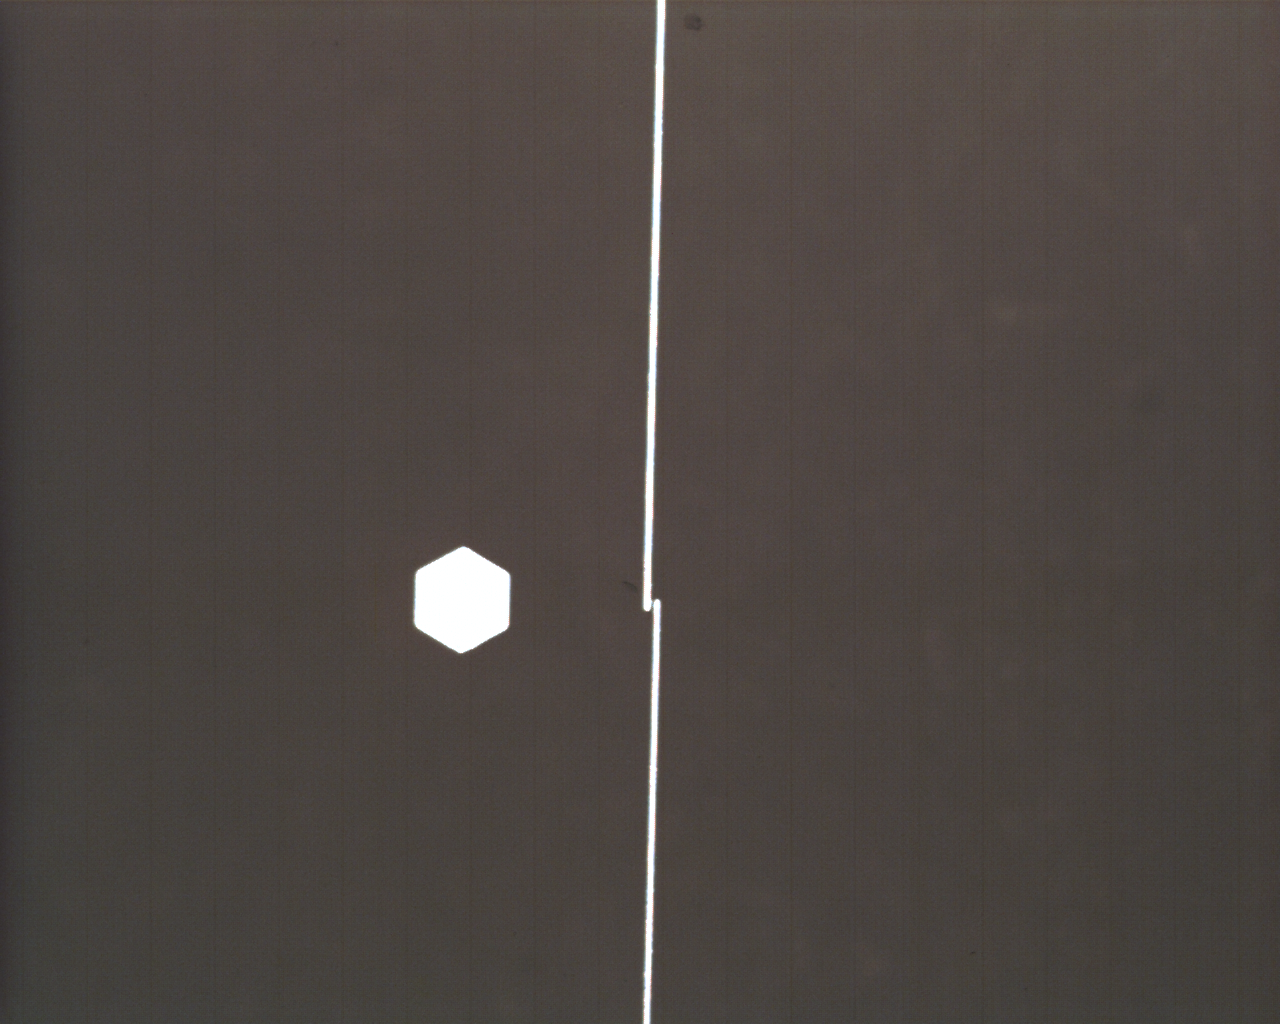
\includegraphics[width=\textwidth]{images/goodElectrode.png}
        \caption{Impedance magnitude and phase}
    \end{subfigure}
    \hfill
    \begin{subfigure}[b]{0.45\textwidth}
        \centering
        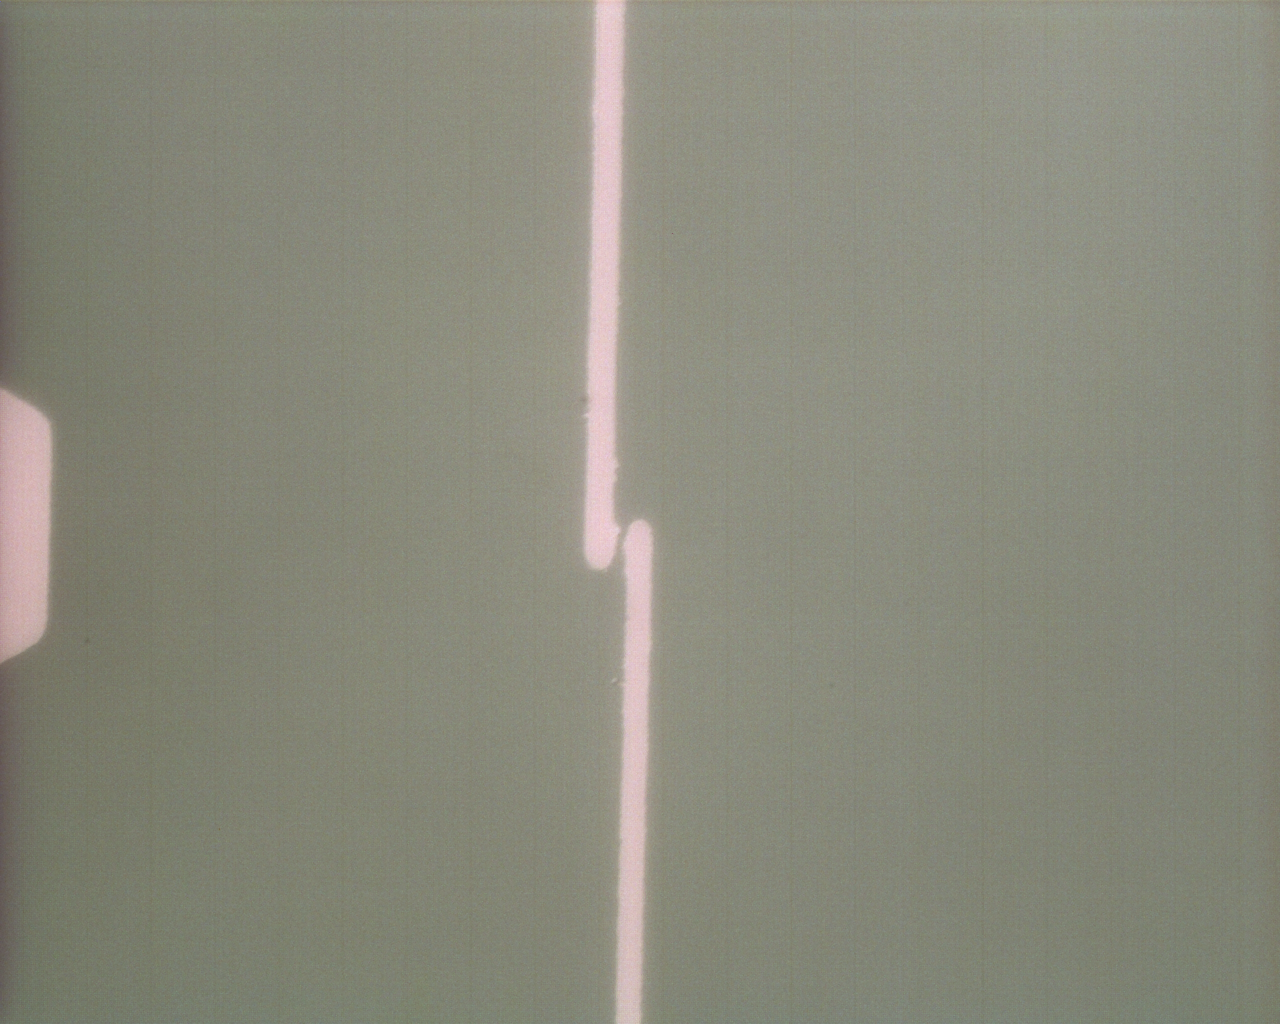
\includegraphics[width=\textwidth]{images/goodElectrodeCloseUp.png}
        \caption{Real and imaginary impedance}
    \end{subfigure}
\end{figure}


\FloatBarrier

\subsection{Device Bonding}


\begin{figure}[h]
    \centering
    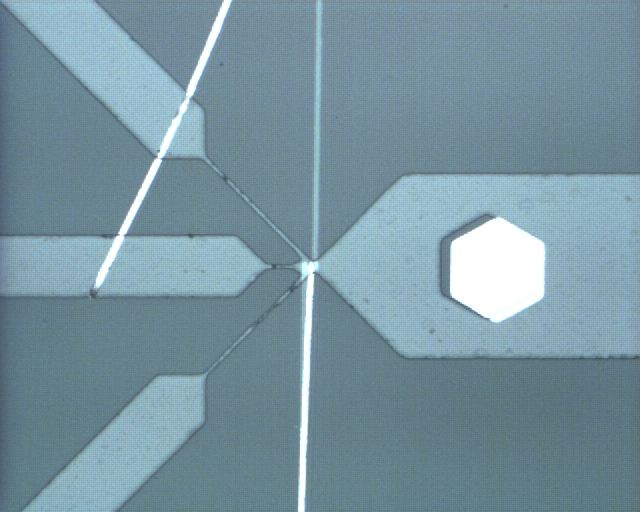
\includegraphics[width=\textwidth]{images/bad_device.png}
    \caption{Failed device}
    \label{fig:bad_device}
\end{figure}


\begin{figure}[h]
    \centering
    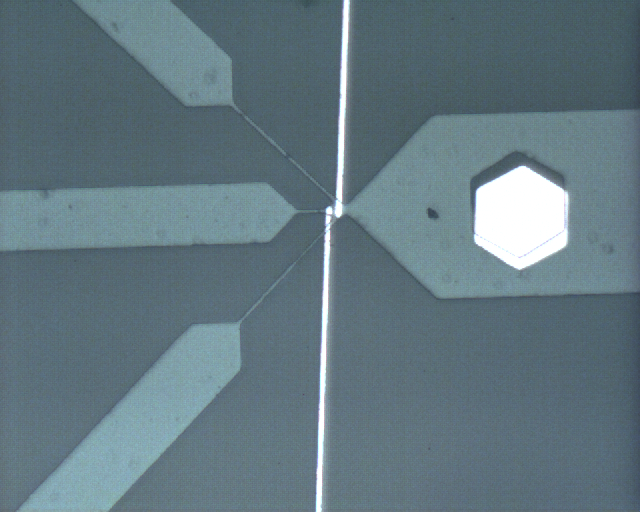
\includegraphics[width=\textwidth]{images/good_device.png}
    \caption{Good device}
    \label{fig:good_device}
\end{figure}

\FloatBarrier

\section{Impedance Spectroscopy System}

\begin{figure}[h]
    \centering
    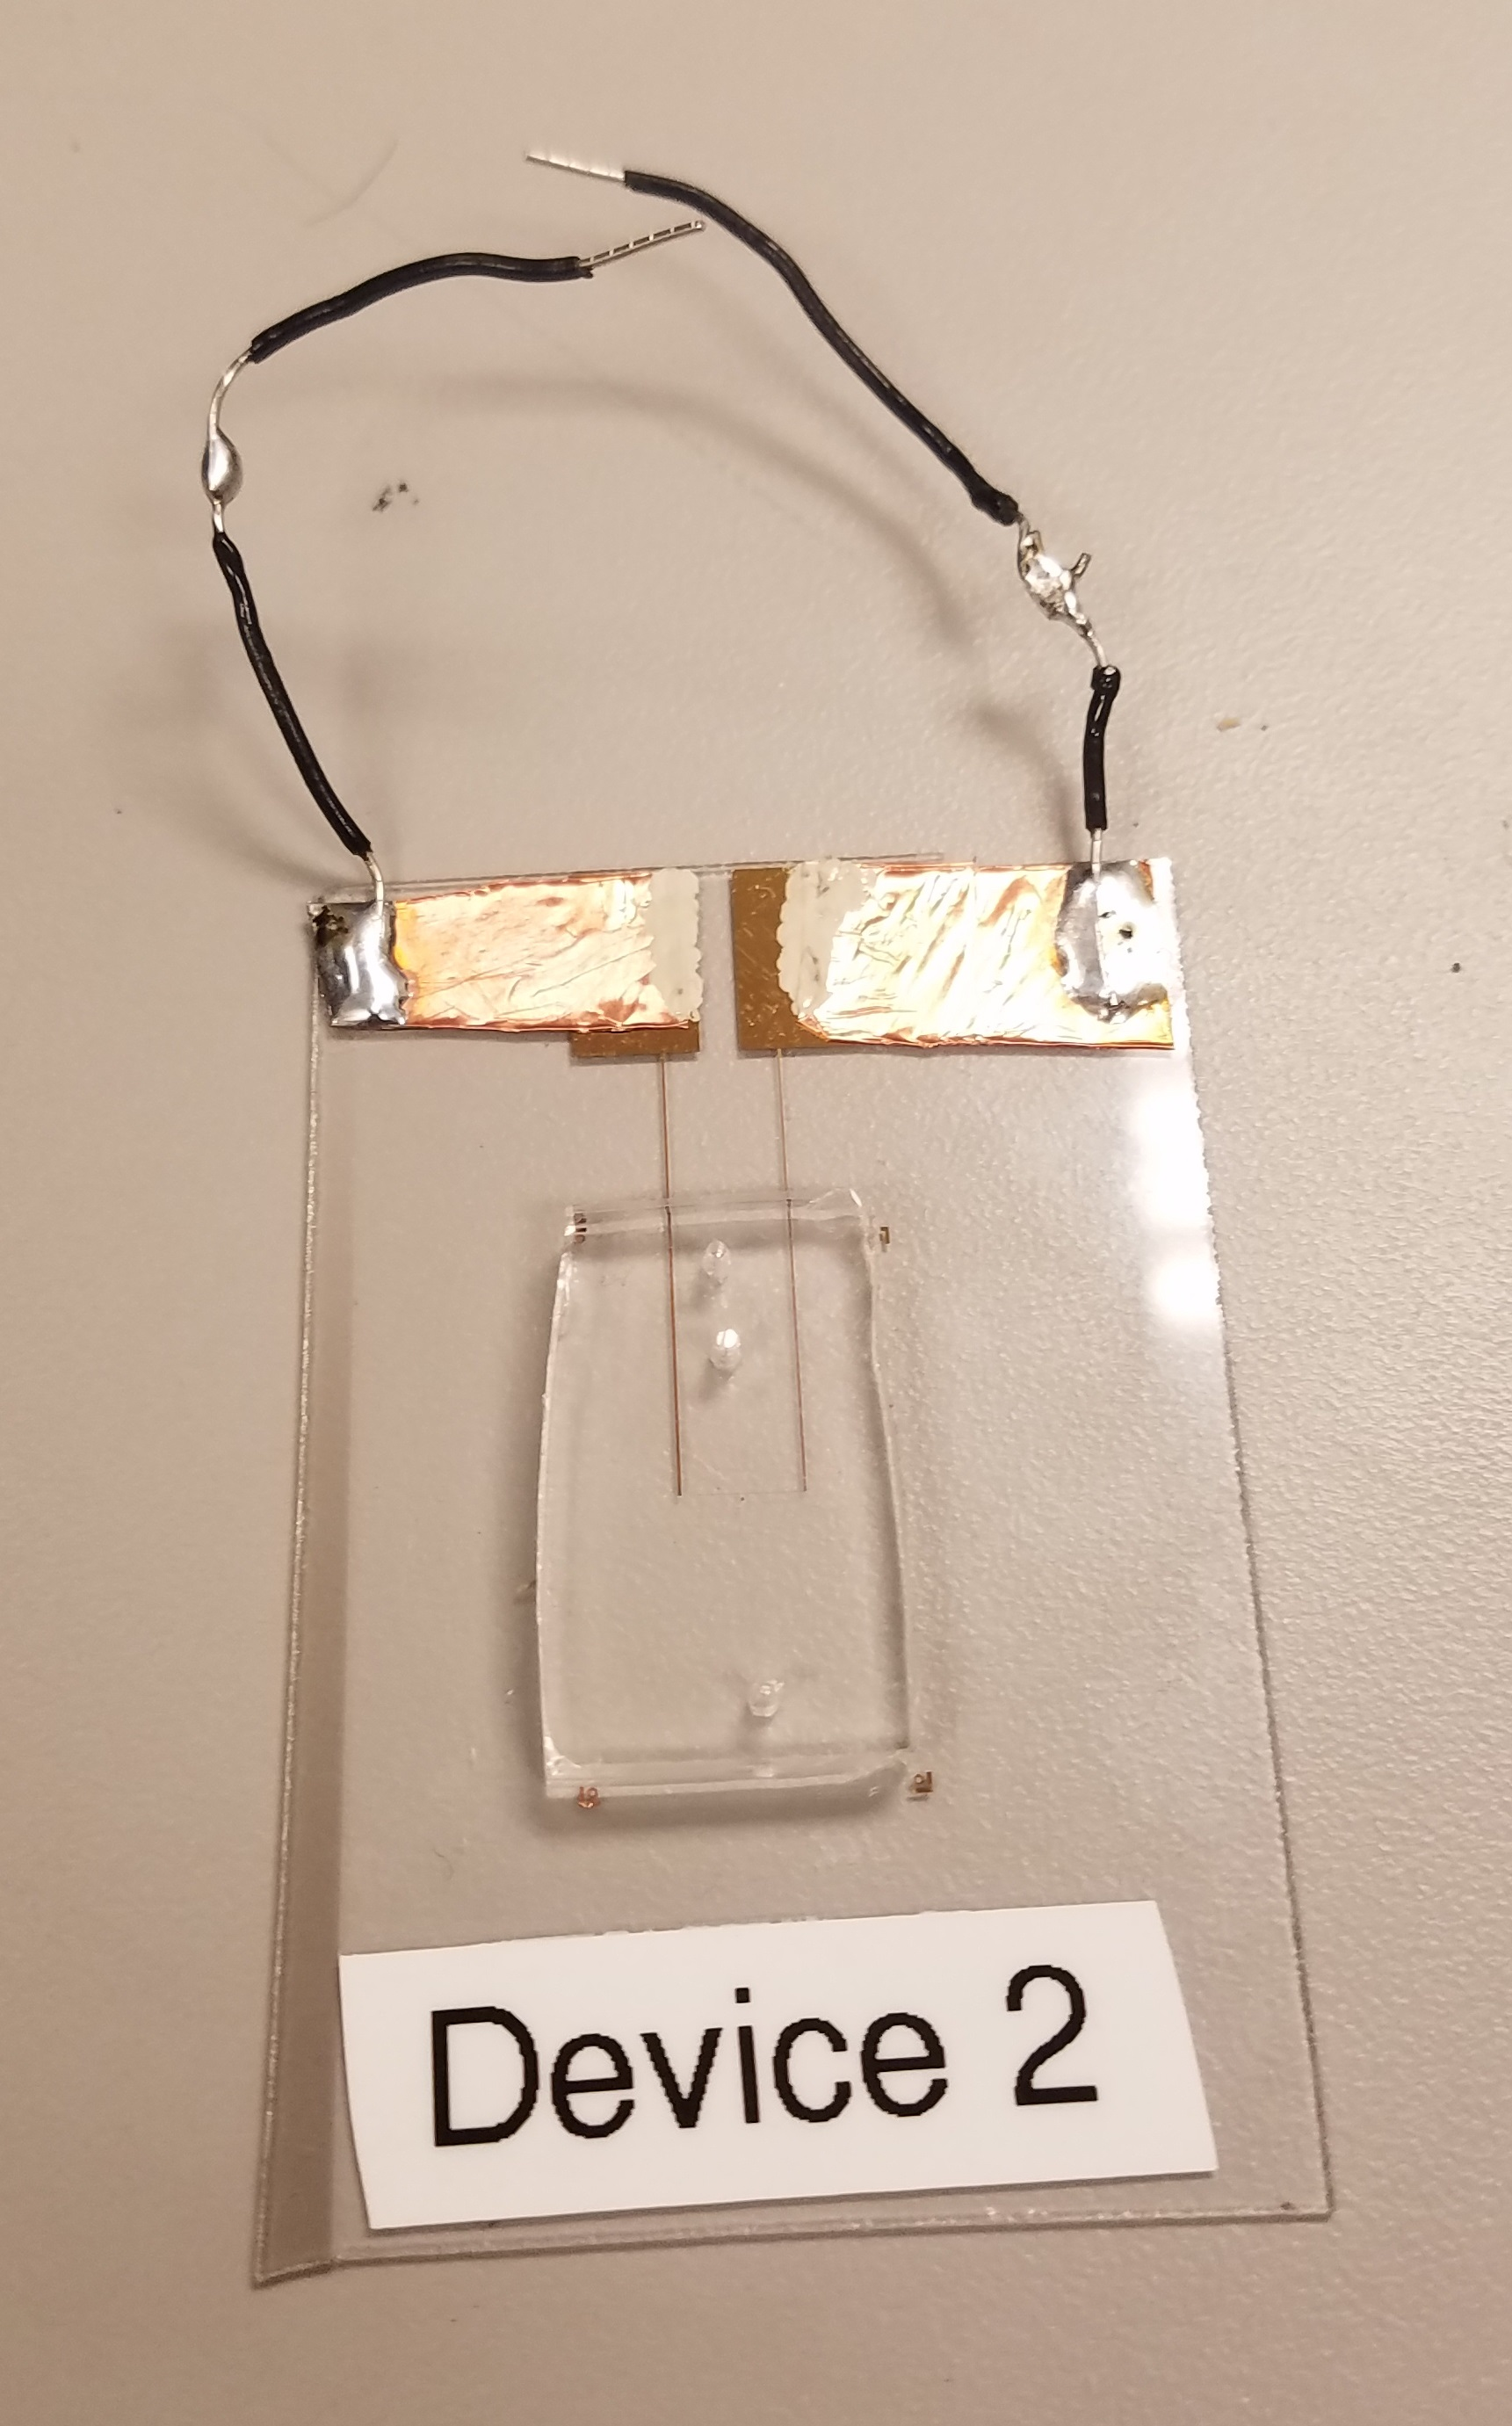
\includegraphics[width=0.5\textwidth]{images/device_22.jpg}
    \caption{Device two}
    \label{fig:my_label}
\end{figure}

\begin{figure}[h]
    \centering
    \begin{subfigure}[b]{0.45\textwidth}
        \centering
        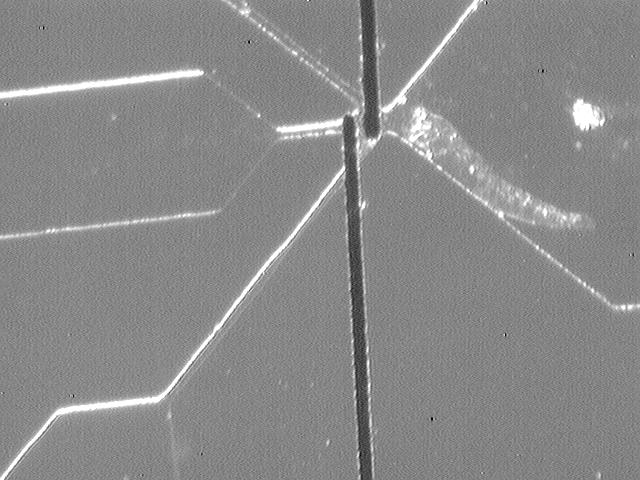
\includegraphics[width=\textwidth]{images/IS_empty.jpg}
        \caption{Sensor chamber fluid filled}
    \end{subfigure}
    \hfill
    \begin{subfigure}[b]{0.45\textwidth}
        \centering
        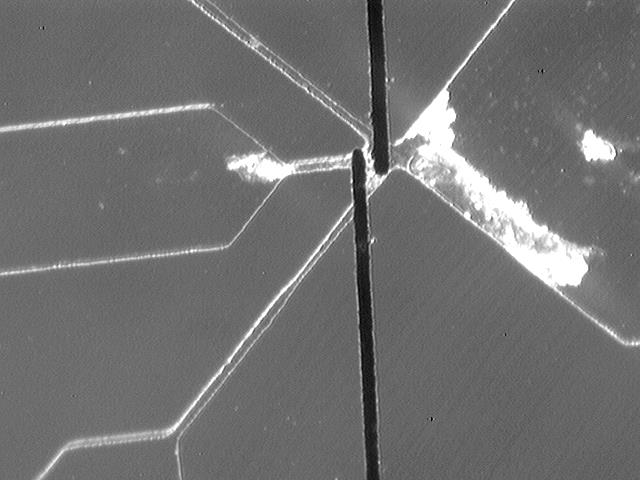
\includegraphics[width=\textwidth]{images/IS_particle_saturation.jpg}
        \caption{Sensor chamber 7$\mu$m }
    \end{subfigure}
    \\
    \vspace{0.1 in}
    \begin{subfigure}[b]{0.45\textwidth}
        \centering
        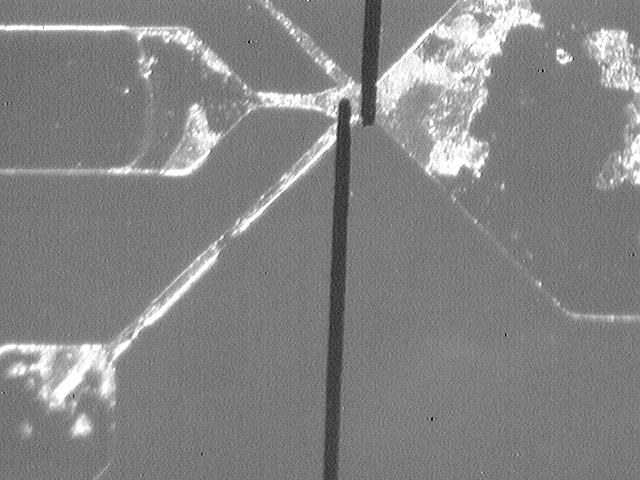
\includegraphics[width=\textwidth]{images/IS_jammed.jpg}
        \caption{Jammed}
    \end{subfigure}
    \hfill
    \begin{subfigure}[b]{0.45\textwidth}
        \centering
        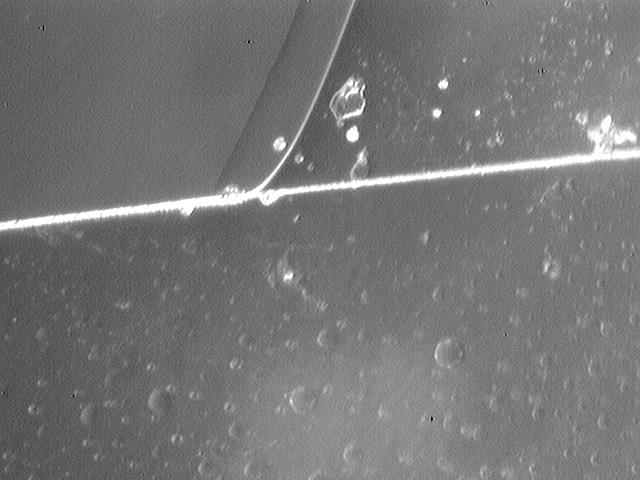
\includegraphics[width=\textwidth]{images/IS_device_delamination.jpg}
        \caption{Device delamination}
    \end{subfigure}
    \caption{IS device sensor region images.}
    \label{fig:IS_sensor_reigon_measurement}
\end{figure}

\begin{figure}[h]
    \centering
    \begin{subfigure}[b]{\textwidth}
        \centering
        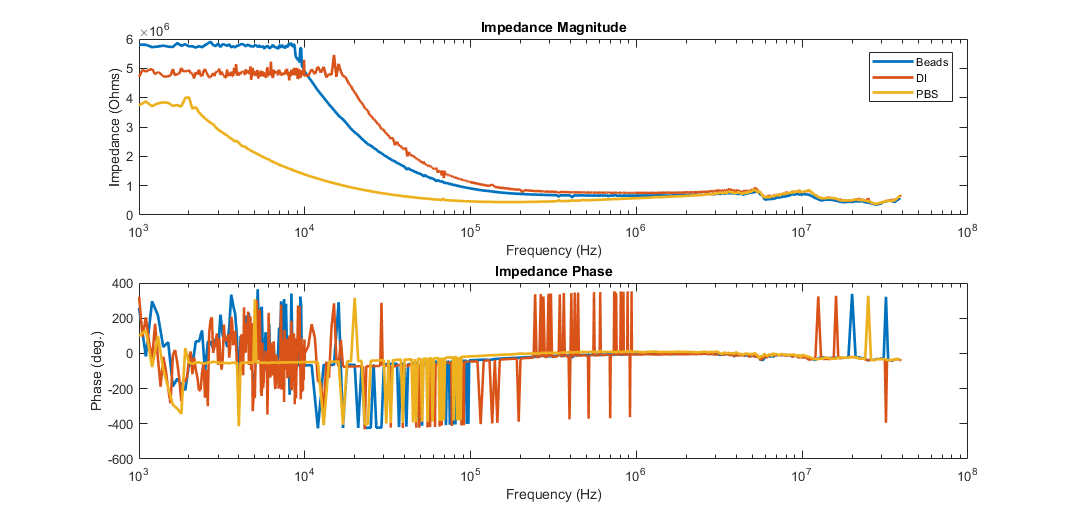
\includegraphics[width=\textwidth]{images/raw_IS_data_mag_phase.png}
        \caption{Sensor chamber fluid filled}
    \end{subfigure}
    \\
    \vspace{0.1 in}
    \begin{subfigure}[b]{\textwidth}
        \centering
        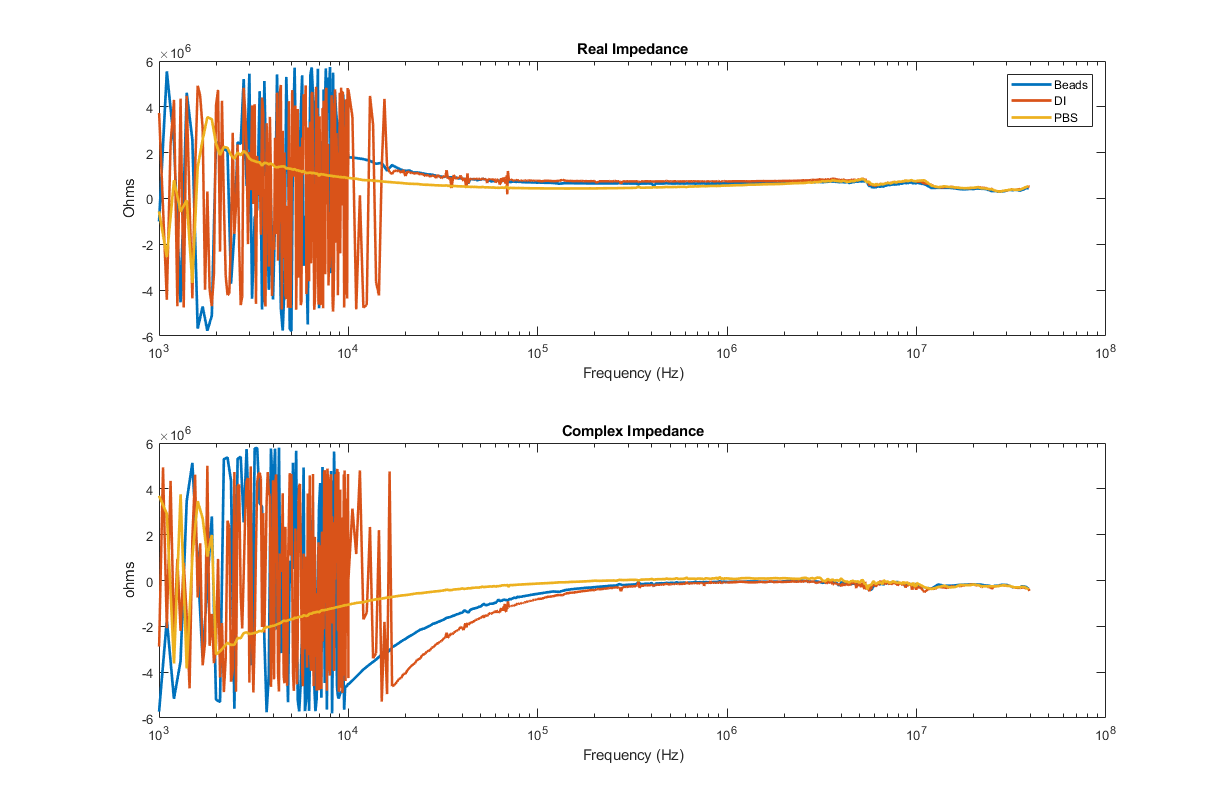
\includegraphics[width=\textwidth]{images/raw_IS_data_real_imag.png}
        \caption{Sensor chamber 7$\mu$m }
    \end{subfigure}
    \\
    \vspace{0.1 in}
    \begin{subfigure}[b]{\textwidth}
        \centering
        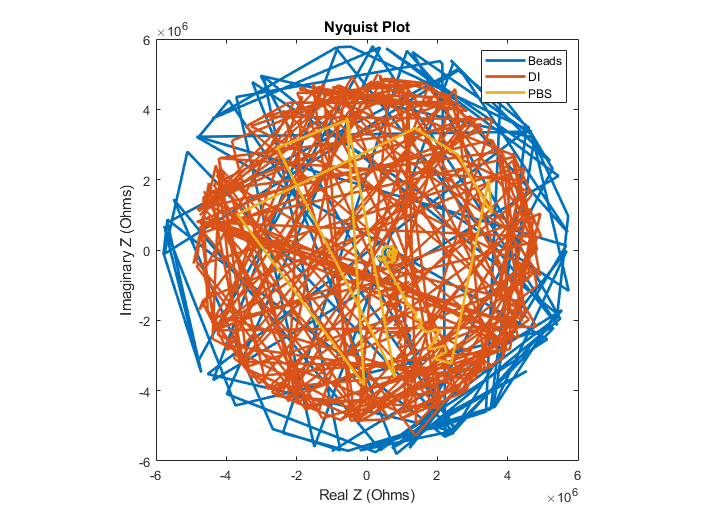
\includegraphics[width=\textwidth]{images/raw_IS_data_nyquist.png}
        \caption{Jammed}
    \end{subfigure}
    \caption{IS device sensor region images.}
    \label{fig:IS_data_raw}
\end{figure}


\FloatBarrier

\section{Modeling}


\section{Spice Model/Measurement analysis}
